% =====================================================================
% OPTIONAL SUPPLEMENTARY MATERIAL (goes after the AI Ethics Statement, per the brief)
% Generated from results/ by a script (numbers copied, not retyped). Needs \usepackage{float} for [H].
% =====================================================================
\subsection*{A. Learning-rate selection (validation set \texttt{fsl\_val\_rl})}
\begin{table}[H]\centering\small
\begin{tabular}{lccc}\toprule
Base, gen 0 & val.\ loss & SE & in-context acc.\\\midrule
$10^{-5}$ (used) & 0.0248 & 0.0025 & 0.997\\
$3{\times}10^{-6}$ & 0.3765 & 0.0119 & 0.841\\
$3{\times}10^{-5}$ & 0.0016 & 0.0007 & 1.000\\
\bottomrule\end{tabular}\\[6pt]
\begin{tabular}{lcccc}\toprule
Extended, gen 0 & total loss & symbol loss & query acc. & next-label acc.\\\midrule
$10^{-5}$ & 1.374 & 1.083 & 0.956 & 0.953\\
$3{\times}10^{-5}$ & 0.876 & 0.787 & 0.985 & 0.991\\
$10^{-4}$ (used) & 0.796 & 0.757 & 0.991 & 0.996\\
$3{\times}10^{-4}$ & 12.013 & 0.758 & 0.694 & 0.652\\
\bottomrule\end{tabular}
\caption{Validation results after $10^6$ sequences. The symbol-loss floor for $p{=}0.5$ is $\ln 2\approx0.693$.}
\end{table}

\subsection*{B. Early-warning test for the strongest induction head ($m_{\max}$)}
First generation at which each measure is worse than generation 0 by more than $z$ paired standard
errors, and the first at which it changes by more than 10\%; ``--'' means never within the run.
\begin{table}[H]\centering\small
\begin{tabular}{llccccc}\toprule
Condition & Behaviour & $z{=}2$ & $z{=}3$ & $z{=}5$ & $>10\%$ & $m_{\max}$ at $>10\%$\\
 & & circ./beh. & circ./beh. & circ./beh. & beh. & \\\midrule
$T{=}2$ & accuracy & 1/1 & 1/1 & 1/2 & 3 & 3\\
 & loss & 1/1 & 1/1 & 1/1 & 1 & 3\\
 & use-context & 1/1 & 1/1 & 1/1 & 2 & 3\\
\midrule
$T{=}2$, 10\% real & accuracy & 1/1 & 1/1 & 1/2 & 3 & 3\\
 & loss & 1/1 & 1/1 & 1/1 & 1 & 3\\
 & use-context & 1/1 & 1/1 & 1/1 & 3 & 3\\
\midrule
$T{=}1$ & accuracy & 1/1 & 1/2 & 1/8 & -- & 8\\
 & loss & 1/1 & 1/1 & 1/1 & 1 & 8\\
 & use-context & 1/1 & 1/1 & 1/1 & -- & 8\\
\midrule
argmax & accuracy & --/-- & --/-- & --/-- & -- & --\\
 & loss & --/-- & --/-- & --/-- & -- & --\\
 & use-context & --/-- & --/-- & --/-- & -- & --\\
\midrule
$T{=}2$, lr $3{\times}10^{-5}$ & accuracy & & 4/4 & & 4 & 4\\
 & loss & & 4/1 & & 1 & 4\\
 & use-context & & 4/1 & & 3 & 4\\
\midrule
ext.\ $T{=}1$ & accuracy & & 1/-- & & -- & 1\\
 & loss & & 1/-- & & 2 & 1\\
 & use-context & & 1/1 & & -- & 1\\
\midrule
ext.\ argmax & accuracy & & --/-- & & -- & --\\
 & loss & & --/-- & & 2 & --\\
 & use-context & & --/1 & & -- & --\\
\bottomrule\end{tabular}
\caption{Lower block: only $z{=}3$ was run. In the extended version a 10\% change in loss is a change of
about 0.002 (loss $\approx0.02$), so that column is not meaningful there.}
\end{table}

\subsection*{C. Extended version, $T{=}1$: next-symbol drift}
\begin{table}[H]\centering\small
\begin{tabular}{rcccccc}\toprule
Pool & out-of-context & repeat share & spread (obs.) & spread if & spread if & corr.\ with own\\
gen & symbols & (in context) & & generalising & memorising & training share\\\midrule
0 & 0.000 & 0.500 & 0.022 & 0.021 & 0.021 & --\\
1 & 0.020 & 0.515 & 0.041 & 0.022 & 0.041 & 0.03\\
2 & 0.034 & 0.522 & 0.058 & 0.022 & 0.058 & 0.57\\
4 & 0.058 & 0.543 & 0.081 & 0.023 & 0.089 & 0.82\\
6 & 0.078 & 0.558 & 0.092 & 0.023 & 0.114 & 0.86\\
8 & 0.097 & 0.568 & 0.102 & 0.024 & 0.135 & 0.88\\
10 & 0.114 & 0.572 & 0.109 & 0.024 & 0.152 & 0.90\\
\bottomrule\end{tabular}
\caption{Pool $g$ is written by model $g{-}1$. Spread: variance across sequences of the share of copies
whose next symbol repeats the query (about 12.8 copies per sequence).}
\end{table}

\subsection*{D. Generation-0 heads}
\begin{figure}[H]\centering
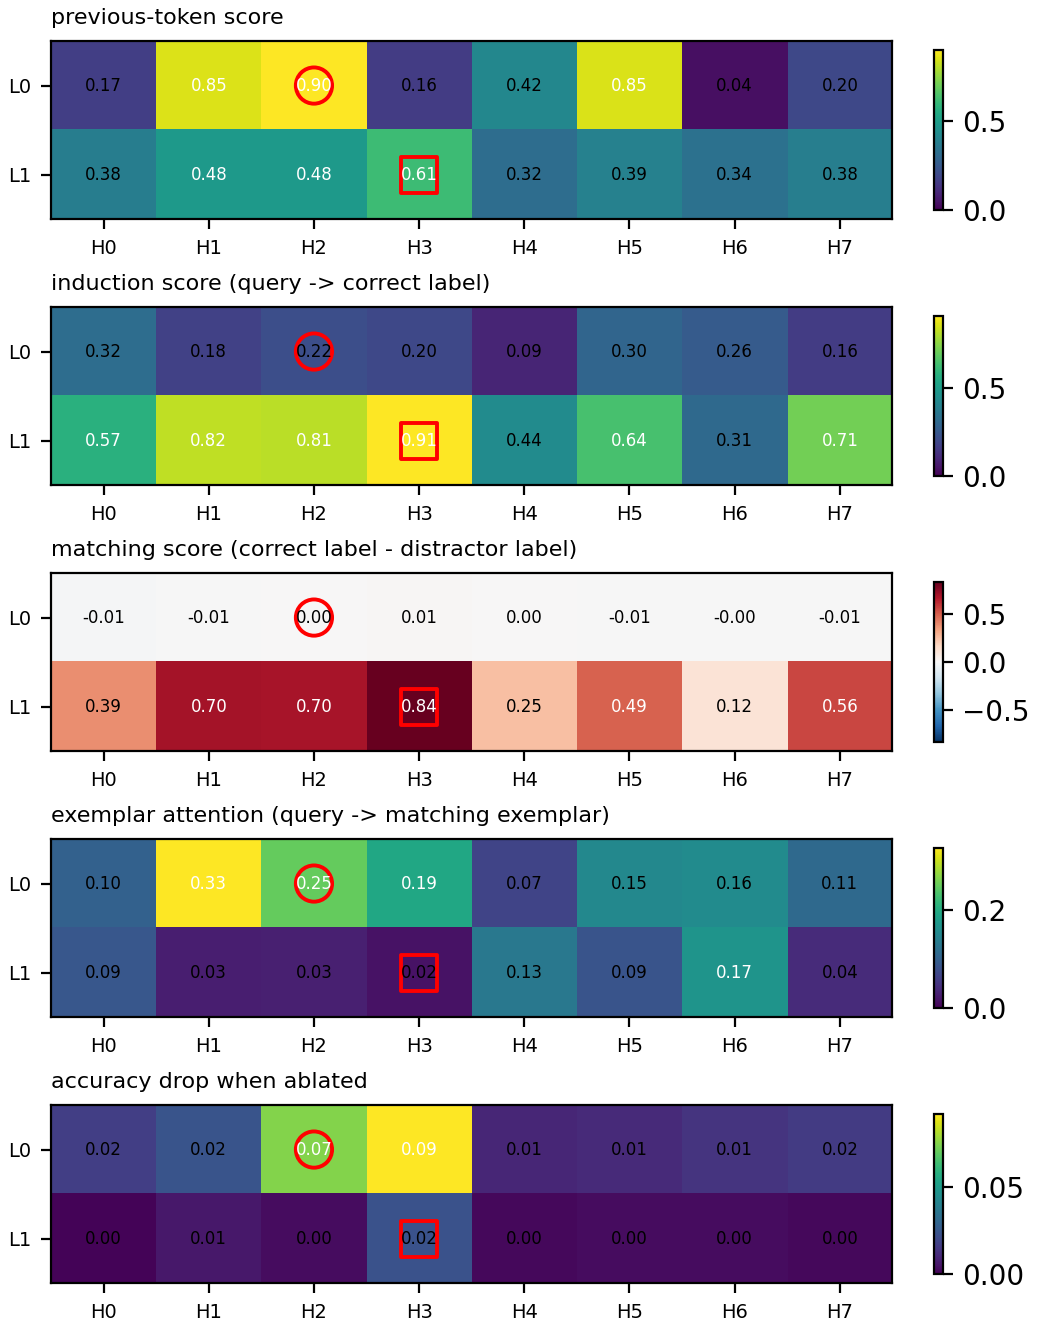
\includegraphics[width=0.48\linewidth]{gen0_head_heatmaps_base.png}\hfill
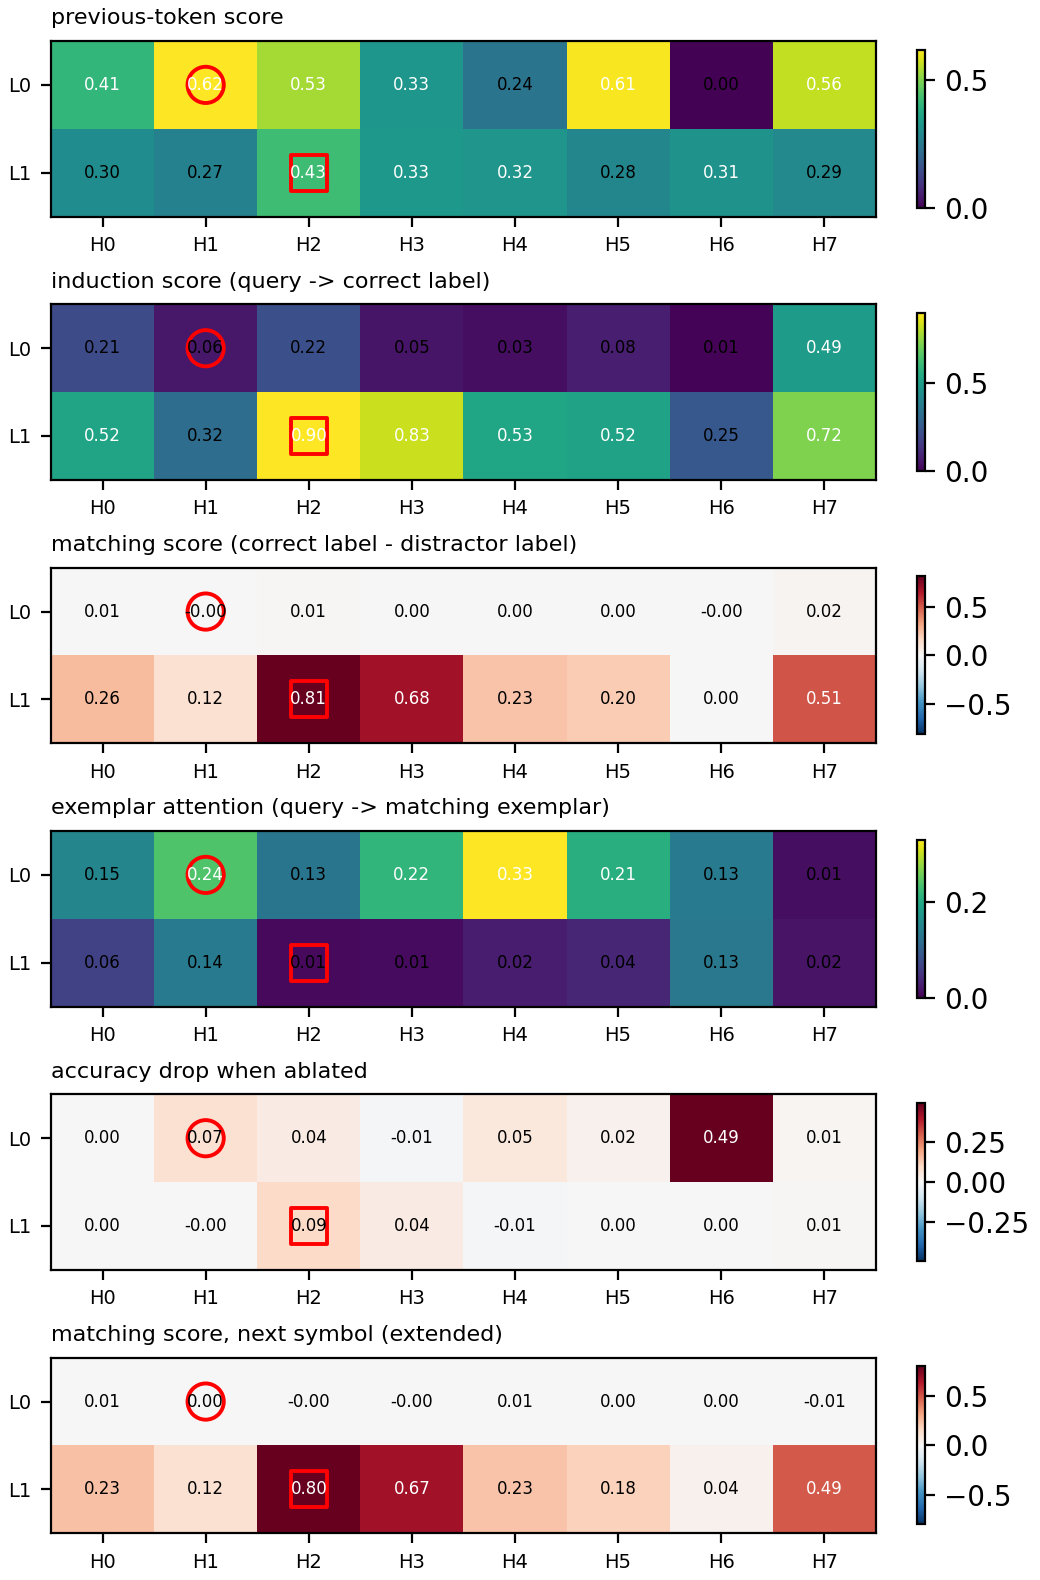
\includegraphics[width=0.48\linewidth]{gen0_head_heatmaps_ext.png}
\caption{Head scores and single-head ablation of the generation-0 model, base (left) and extended
(right). Circle: chosen previous-token head; square: chosen induction head.}
\end{figure}

\subsection*{E. Accuracy on the training, validation and test sets}
\begin{table}[H]\centering\small
\begin{tabular}{lcccc}\toprule
Run (final checkpoint) & train & validation & train chars., new exemplars & test (held-out chars.)\\\midrule
base generation 0 & 1.000 & 0.997 & 0.865 & 0.958\\
base $T{=}2$, generation 10 & 0.531 & 0.495 & 0.498 & 0.496\\
base $T{=}2$ (10\% real), generation 10 & 0.508 & 0.469 & 0.514 & 0.498\\
base $T{=}1$, generation 10 & 0.997 & 0.954 & 0.866 & 0.934\\
base argmax, generation 3 & 1.000 & 0.997 & 0.865 & 0.958\\
base generation 0, lr $3{\times}10^{-5}$ & 1.000 & 1.000 & 0.898 & 0.974\\
extended generation 0 & 1.000 & 0.991 & 0.863 & 0.973\\
extended $T{=}1$, generation 10 & 0.998 & 0.992 & 0.876 & 0.986\\
\bottomrule\end{tabular}
\caption{In-context accuracy from the training logs (\texttt{fsl\_train}, \texttt{fsl\_val\_rl},
\texttt{fsl\_train\_valex}, \texttt{fsl\_test\_class}); source \texttt{results/test\_metrics.csv}.
Chance is 0.5. The test set confirms the validation results: collapsed models are at chance on unseen
characters too.}
\end{table}
